Individual part of Kim A. Jakobsen.

\subsection{Existing applications}
At the current state of technology fingerprinting, using WI-FI, is the most promising.
There are several reasons why this is true, I now discuss the most relevant of them.

\subsubsection{\qquad Use Scenarios} 
Indoor positioning is a relative new technology and I do not believe we can imagine what we will use it for in the furniture.
However, in the near future the technology is going to be used in museums, shopping malls, airports, and other large buildings.
These guess is based on what the industry is currently doing.

Qubulus indoor positioning is a company that offer indoor positioning using WI-FI fingerprinting~\cite{qubulus}.
They do not state how they generate the radio map but they show a image, see Figure~\ref{fig:qubulus} that looks like the result of traditional generation of a radio map.
One of their use cases is usage in shopping malls.
By tracking where customers go it is possible to make improvement in the shopping mall to the end of improving the shopping experience of the customers.
This is an example of indoor position service used by the the company to indirectly improve the experience of the shopping mall.

Wifarer also offers WI-FI based indoor positioning~\cite{wifarer}.
To create a radio map Wifarer shows up at your location and use their special "`calibration software"'.
One of their use cases is usage in a museum.
They offer visitors location specific content such as information about an exhibition item.
This is an example of indoor position service directly target to visitors to give them a better experience.

Both these companies offer indoor positioning services that are similar to outdoor positioning systems.
I think this is an important fact.
Outdoor position services such as GPS gives the user a point where they are located.
People expect it have a service that functions like they are use to, which means that a service that places them in a cell, e.g. a room, they want the same accuracy they are use to.
WI-FI based fingerprinting is GPS like and gives the user a point where they are located.
That is one of the reasons that make be believe that WI-FI based indoor positioning is going to dominate the future.  
\begin{figure}%
\centering
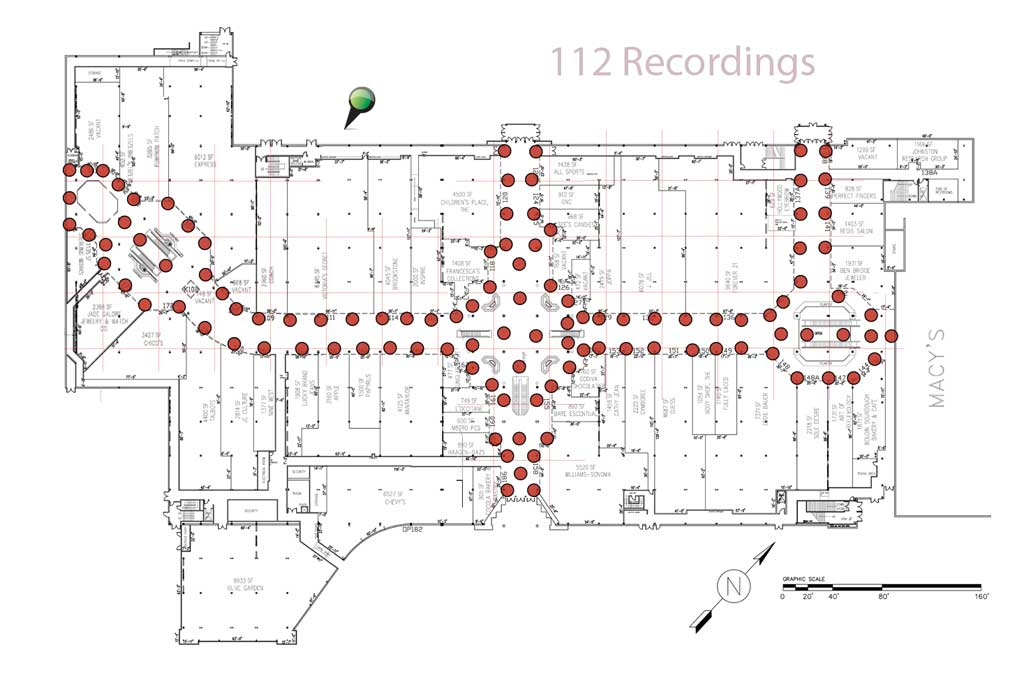
\includegraphics[width=\columnwidth]{images/USA_Stonestown_Recordings-shrunk.jpg}%
\caption{Map of the locations inserted into the radio map. This illustration originates from~\cite{qubulus}.}%
\label{fig:qubulus}%
\end{figure}



\subsubsection{\qquad Alternative Technologies} 
In our shared part describe the Graph Model Based, Fingerprinting, and Hybrid of the two techniques.
The Graph Model Based have its strength in its partitioning of locations and in robustness in relation to interference.
While one of its greatest strengths then is the partitioning also one of its greatest weaknesses. 
As mentioned then people expect get a point and not an area.
I deem that this is going to be a problem in the adoption of this technique.  
Large open indoor locations, e.g. museums, are hard to partition into smaller cell.
Due to this difficulty it is hard to apply to the the industrial world.

Hybrid of fingerprinting and Graph Model Based technique have some of the best results in tests. 
But it do not have any extra advantages that cannot be achieved with WI-FI based fingerprinting.

\subsubsection{\qquad Improving WI-FI Fingerprinting} 
As mention then WI-FI fingerprinting have several drawbacks witch need to be addressed.
We explained the general process in Section \ref{sub:radiomap} and I do not explain it further.
The first weakness I want to address is the demanding setup process.
The setup often require manual labour in some degree.
A solution to this is to have a tool which models the location encompassing wall material, router type, and people density. 
This tool would then generate a complete set of radio maps, such that there is coverage for every location in the building, this, however, creates a new problem of searching the now large radio maps. 
The model should be self improving. 
Radio maps are improve when actual number of visitors are known, this is important because more people creates more inference and this need to be accounted for. 
To further improve the radio maps a few wireless receives should be place in the building, they constant measure the radio signal strength and adjust or switch to a more fitting radio map.
This self improvement also counters the second weakness, the changing level if inference.
Depending of how many people with mobile phones are in the area, if doors are open or closed, and temperature of the location.
If a location have many visitors it might be necessary to have a sets of radio maps.
The most appropriate radio maps should be used.

\subsubsection{\qquad The Future of Indoor Location Based Services}
No matter which technology is going to dominate the near future then there is the question of privacy.
The Wifarer museum use case do not pose any direct threads to the privacy of the visitors.
The shopping mall use case from Qubulus do.
The instant that someone wants to analyse the data, the customers privacy is a relevant question.
If a customer feels that hers privacy is threatened she might chose not to shop in the shopping center.
She might also disable her mobile device and therefore not be detected as present by the system.
This might pose a great problem is someone want an accurate count of how many enters a location.
This desire might spawn a new branch of indoor position that is able to track people by use of infrared or other technologies that do not require the participation of the customer.
